\section{Methods}
\label{sec:methods}

In this manuscript, we are primarily concerned with $k$-NN search in a finite-dimensional space.
Given a dataset $\textbf{X} = \{x_1 \dots x_n\}$ of cardinality $|\textbf{X}| = n$, we define a \textit{point} or \textit{datum} $x_i \in \textbf{X}$ as a singular observation. Examples include the neural-network embedding of an image, the genome of an organism, and a measurement of a radio frequency signal.

We define a \textit{distance function} $f : \textbf{X} \times \textbf{X} \mapsto \mathbb{R}^+ \ \cup \ \{0\}$ which, given two points, deterministically returns a finite and non-negative real number.
A distance of zero defines identity among points (i.e.,\,$f(x, y) = 0 \Leftrightarrow x = y$) and larger values indicate greater dissimilarity among points.
We also require that the distance function be symmetric (i.e.,\,$f(x, y) = f(y, x) \ \forall \ x, y \in \textbf{X}$).
In addition to these constraints, if the distance function obeys the triangle inequality (i.e.,\,$f(x, y) \leq f(x, z) + f(z, y) \ \forall \ x, y, z \in \textbf{X}$), then it is also a \textit{distance metric}.
Similar to~\cite{yu2015entropy}, when used with distance metrics, all search algorithms in CAKES are exact.
For example, Euclidean, Levenshtein~\cite{levenshtein1966binary} and Dynamic Time Warping (DTW)~\cite{muller2007dynamic} distances are all distance metrics, while cosine distance is not a metric because it violates the triangle inequality (e.g.,\,consider the points $x = (1, 0)$, $y = (0, 1)$ and $z = (1, 1)$ on the Cartesian plane).

The choice of an appropriate distance function varies by dataset and domain.
For example, with neural-network embeddings, one could use Euclidean (L2) or cosine distance.
With genomic or proteomic sequence data, Levenshtein or Hamming distance is useful.
With time-series data, one could use Dynamic Time Warping (DTW) or Wasserstein distance.

CAKES derives its advantages from the manifold hypothesis~\cite{fefferman2016testing}, the notion that high-dimensional data collected from constrained generating phenomena typically only occupy a low-dimensional manifold within their embedding space.
We say that such data are \textit{manifold-constrained} and have low \textit{local fractal dimension} (LFD).
In other words, we assume that the dataset is embedded in a $D$-dimensional space, but that the data only occupy a $d$-dimensional manifold, where $d \ll D$.
While we sometimes use Euclidean notions to describe the geometric and topological properties of the clusters and manifold, CLAM and CAKES do not rely on such notions;
they serve merely as convenient and intuitive vocabulary to discuss the underlying mathematics.
CAKES exploits the low LFD of such datasets to accelerate search.
We define LFD at some length scale around a point in the dataset as:
\begin{equation}
    \text{LFD}(q, r_1, r_2) = \frac{\text{log} \left( \frac{|B(q, r_1)|}{|B(q, r_2)|} \right) }{\text{log} \left( \frac{r_1}{r_2} \right) }
    \label{eq:methods:lfd-original}
\end{equation}
where $B(q, r)$ is the set of points contained in the metric ball of radius $r$ centered at a point $q$ in the dataset $\textbf{X}$.

We use a simplified version of Equation~\ref{eq:methods:lfd-original} by using a length scale where $r_1 = 2 \cdot r_2$.
\begin{equation}
    \text{LFD}(q, r) = \text{log}_2 \left( \frac{|B(q, r)|}{|B(q, \frac{r}{2})|} \right)
    \label{eq:methods:lfd-half}
\end{equation}

Intuitively, LFD measures the rate of change in the number of points in a ball of radius $r$ around a point $q$ as $r$ increases. When the vast majority of points in the dataset have low ($\ll D$) LFD, we can simply say that the dataset has low LFD.
We stress that this concept differs from the \textit{embedding dimension} of a dataset.
To illustrate the difference, consider the SILVA 18S rRNA dataset that contains genomic sequences with unaligned lengths of up to 3,718 base pairs and aligned length of 50,000 base pairs.
Hence, the \textit{embedding dimension} of this dataset is at least 3,718 and at most 50,000.
However, physical constraints (namely, biological evolution and biochemistry) constrain the data to a lower-dimensional manifold within this space.
LFD is an approximation of the dimensionality of that lower-dimensional manifold in the ``vicinity'' of a given point.
Figure~\ref{fig:results:lfd-plots} illustrates this concept on a variety of datasets, showing how real datasets uphold the manifold hypothesis.
For real-world datasets, we expect the LFD to be locally uniform, i.e.,\,when $r$ is small, but potentially highly variable at larger length scales, i.e.,\,when $r$ is large.


\subsection{Clustering}
\label{sec:methods:clustering}

We define a \textit{cluster} as a set of points with a \textit{center} and a \textit{radius}.
The center is the geometric median of the points in the cluster, i.e.,\,it is the point that minimizes the sum of distances to all other points in the cluster.
In cases where the cardinality of the cluster is large, we take a random subsample of $\sqrt{|C|}$ points and compute the geometric median of that subsample~\cite{ishaq2019clustered}.
The center, therefore, is one of the points in the cluster and is used as a representative of the cluster.
The radius is the maximum distance from the center to any point in the cluster.
Each non-leaf cluster has two child clusters in much the same way that a node in a binary tree has two child nodes.
Note that clusters can have overlapping volumes and, in such cases, points in the overlapping volume are assigned to exactly one of the overlapping clusters.
As a consequence, a cluster can be a proper subset of the metric ball at the same center and radius, i.e.,\,$C(c, r) \subset B(c, r)$. We denote the cluster tree by $\mathcal{T}$ and the root by $\mathcal{R}$ (see Section~\ref{sec:methods:clustering:building-the-tree}).

Hereafter, when we refer to the LFD of a cluster, it is estimated at the length scale of the cluster radius and half that radius, i.e.,\,using Equation~\ref{eq:methods:lfd-half}.
We also only use points that are in $C(c, r)$ instead of all those in $B(c, r)$.

The \textit{metric entropy} $\mathcal{N}_{r}(X)$ for some radius $r$ is the minimum number of clusters of a uniform radius $r$ needed to cover the data~\cite{yu2015entropy} for a flat clustering with clusters of radius $r$.
In this paper, where the clustering is hierarchical rather than flat, we define the metric entropy $\mathcal{N}_{\hat{r}}(X)$ as the number of leaf clusters in the tree where $\hat{r}$ is the mean radius of all leaf clusters.


\subsubsection{Building the Tree}
\label{sec:methods:clustering:building-the-tree}

We start by performing a divisive hierarchical clustering on the dataset using CLAM to obtain a cluster tree $\mathcal{T}$.
The procedure is almost identical to that outlined in CHESS~\cite{ishaq2019clustered}, but with better selection of poles for partitioning (see Algorithm~\ref{alg:methods:partition}).
After building $\mathcal{T}$ with CLAM, we also perform a depth-first reordering of the dataset (see Section~\ref{sec:methods:clustering:depth-first-reordering}).

\begin{algorithm} % enter the algorithm environment
    \caption{Partition($C$, $criteria$)} % give the algorithm a caption
    \label{alg:methods:partition} % and a label for \ref{} commands later in the document
    \begin{algorithmic} % enter the algorithmic environment
        \Require $C$, a cluster
        \Require $criteria$, user-specified continuation criteria

        \State $seeds \Leftarrow$ random sample of $\left\lceil \sqrt{|C|} \right\rceil$ points from $C$
        \State $c \Leftarrow$ geometric median of $seeds$
        \State $l \Leftarrow \argmax f(c, x) \ \forall \ x \in C$
        \State $r \Leftarrow \argmax f(l, x) \ \forall \ x \in C$
        \State $L \Leftarrow \{x \ | \ x \in C \land f(l, x) \le f(r, x)\}$
        \State $R \Leftarrow \{x \ | \ x \in C \land f(r, x) < f(l, x)\}$

        \If{$|L| > 1$ \textbf{and} $L$ satisfies $criteria$}
            \State Partition($L$, $criteria$)
        \EndIf

        \If{$|R| > 1$ \textbf{and} $R$ satisfies $criteria$}
            \State Partition($R$, $criteria$)
        \EndIf
    \end{algorithmic}
\end{algorithm}

Given a cluster $C$ with $|C|$ points, we define its two children by the following process. We take a random subsample $S$ of $\sqrt{|C|}$ of $C$'s points, and compute pairwise distances between all points in $S$.
Using these distances, we compute the \textit{geometric median} of $S$; in other words, we find the point that minimizes the sum of distances to all other points in $S$.
We define the \textit{center} of $C$ to be this geometric median.

The \textit{radius} of $C$ is the maximum distance from the center to any other point in $C$.
The point that is responsible for that radius (i.e.,\,the furthest point from the center) is designated the \textit{left pole} and the point that is furthest from the left pole is designated the \textit{right pole}.
We then partition the cluster into a \textit{left child} and a \textit{right child}, where the left child contains all points in the cluster that are closer to the left pole than to the right pole, and the right child contains all points in the cluster that are closer to the right pole than to the left pole.
Without loss of generality, we assign to the left child those points that are equidistant from the two poles.
Starting from a root cluster $\mathcal{R}$ containing the entire dataset, we repeat this procedure until each leaf contains only one datum, or we meet some other user-specified stopping criteria (e.g., minimum cluster radius, minimum cluster cardinality, maximum tree depth, etc).
This process is described in Algorithm \ref{alg:methods:partition}.
During the partitioning process, we also compute (and cache) the LFD of each cluster using Equation~\ref{eq:methods:lfd-half}.


\subsubsection{Depth-First Reordering}
\label{sec:methods:clustering:depth-first-reordering}

In CHESS~\cite{ishaq2019clustered}, each cluster stored a list of indices into the dataset.
This list was used to retrieve the clusters' points during search.
Although this approach allowed us to retrieve the points in constant time, its memory cost was prohibitively high.
With a dataset of cardinality $n$ and each cluster storing a list of indices for its points, we stored a total of $n$ indices at each depth in the tree $\mathcal{T}$.
Assuming $\mathcal{T}$ is balanced, and thus $\mathcal{O}(\log n)$ depth, this approach had a memory overhead of $\mathcal{O}(n \log n)$.
In this work, we introduce a new approach wherein, after building $\mathcal{T}$, we reorder the dataset so that points are stored in a depth-first order.
Then, within each cluster, we need only store its \textit{cardinality} and an \textit{offset} to access its points from the dataset.
The root cluster $\mathcal{R}$ has an offset of zero and a cardinality equal to the number of points in the dataset.
A left child has the same offset its parent, and the corresponding right child has an offset equal to the left child's offset plus the left child's cardinality.
With no additional memory cost nor time cost for retrieving points during search, depth-first reordering offers the same time complexity as CHESS but with $\mathcal{O}(n)$ memory overhead.


\subsubsection{Complexity}
\label{sec:methods:clustering:complexity}

The asymptotic complexity of Partition is the same as described in~\cite{ishaq2019clustered}.
By using an approximate partitioning with a $\sqrt{n}$ sample, we achieve $\mathcal{O}(n)$ cost of partitioning and $\mathcal{O}(n \log n)$ cost of building $\mathcal{T}$.
This is a significant improvement over exact partitioning and tree-building, which cost $\mathcal{O}(n^2)$ and $\mathcal{O}(n^2 \log n)$ respectively.

This complexity analysis ignores the cost of checking the continuation criteria.
While a user could specify criteria of any complexity (our implementation allows for this), for this paper we continue clustering until each cluster is a singleton, i.e.,\,it contains only one point or duplicates of the same point and has a radius of zero.
This criterion costs $\mathcal{O}(1)$ to check per cluster, and so does it not affect the overall complexity of the algorithm as used in this paper.

We also note here that this $\mathcal{O}(n \log n)$ complexity assumes that $\mathcal{T}$ is balanced.
In practice, for real datasets, we expect Algorithm~\ref{alg:methods:partition} to produce anything but a balanced tree; the varying sampling density in different regions of the manifold and the low dimensional ``shape'' of the manifold itself will cause it to be unbalanced.
The only case in which we would expect a balanced tree is if the dataset were uniformly distributed, e.g.,\,in a $d$-dimensional hyper-cube.

When building a tree for a real dataset, the depth would be larger than $\log n$, which would seem to increase the cost of tree-building.
However, because of the large numbers of leaf clusters at shallow depths, each subsequent level of $\mathcal{T}$ would also have fewer points, and so the cost of building each subsequent level would be lower.
Any analysis of unbalanced trees would be highly dependent on the specific dataset, and so we do not provide one here, but we explore empirical results based on forcing a balanced tree in Section~\ref{sec:results:clustering-strategies-and-number-of-distance-computations}.
In any case, the tree is built only once, so this cost is amortized over all search queries and other applications.


\subsection{\texorpdfstring{$k$}{k}-Nearest Neighbors Search}
\label{sec:methods:knn-search}

Given a dataset $\textbf{X}$, a distance function $f$ and the root cluster $\mathcal{R}$ of the tree $\mathcal{T}$ (constructed by Algorithm~\ref{alg:methods:partition}), we can now formally pose the $k$-NN search problem.
Given a user specified integer $k$ and query $q$, $k$-NN search aims to find the $k$ closest points to $q$ in $\textbf{X}$.
In other words, $k$-NN search aims to find the set $H$ such that $|H| = k$ and $H = B_X(q, \rho_k)$ where $\rho_k = \max \left\{ f(q, p) \ \forall \ p \in H \right\}$ is the distance from $q$ to the $k^{th}$ nearest neighbor in $\textbf{X}$.

\begin{figure}[H]
    \centering
    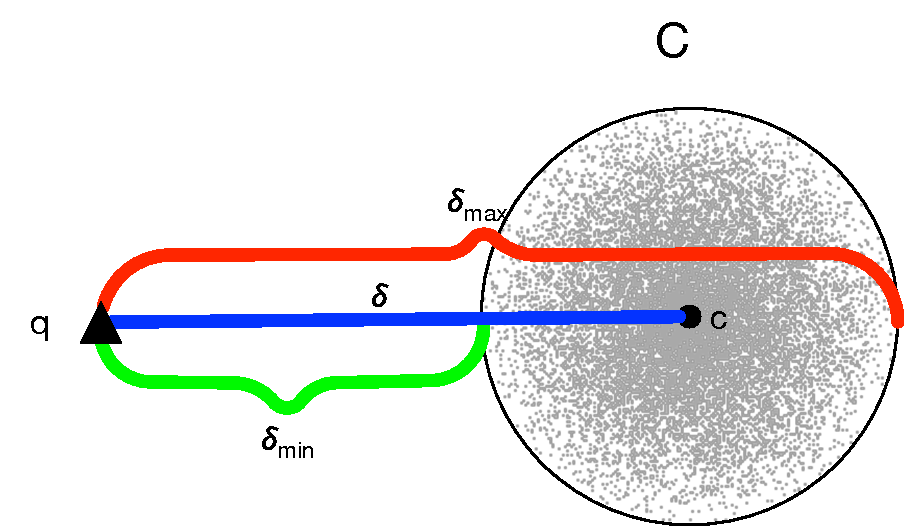
\includegraphics[scale=0.65]{images/geometry/deltas.pdf}
    \caption{
        {\color{blue}$\delta$}, {\color{red}$\delta^{+}$}, and {\color{green}$\delta^{-}$} for a cluster $C$ and a query $q$.
        ${\color{blue}\delta} = f(q, c)$ is the distance from the query to the cluster center $c$.
        ${\color{red}\delta^{+}} = \delta + r$ is the distance from the query to the theoretically farthest point in $C$.
        ${\color{green}\delta^{-}} = \text{max}(0, \delta - r)$ is the distance from the query to the theoretically closest point in $C$.
    }
    \label{fig:methods:deltas}
    \vskip -0.25in
\end{figure}

\begin{minipage}{.425\textwidth}
    \begin{algorithm}[H]
        \caption{tree-search($C$, $q$, $r$)}
        \label{alg:methods:rnn-search:tree-search}
        \begin{algorithmic}
            \Require $C$, a cluster
            \Require $q$, a query
            \Require $r$, a search radius
            \If{$\delta^+_C \leq r$}
                \State \textbf{return} $\{C\}$
            \Else
                \State $[L, R]$ $\Leftarrow$ \textit{children} of $C$
                \State \textbf{return} tree-search($L, q, r$) \\
                \ \ \ \ \ \ \ \ \ \ \ \ \ \ \ $\cup$ tree-search($R, q, r$)
            \EndIf
        \end{algorithmic}
    \end{algorithm}
\end{minipage}
\hfill
\begin{minipage}{.475\textwidth}
    \begin{algorithm}[H]
        \caption{leaf-search($Q$, $q$, $r$)}
        \label{alg:methods:rnn-search:leaf-search}
        \begin{algorithmic}
            \Require $Q$, a set of clusters
            \Require $q$, a query
            \Require $r$, a search radius
            \State $H \Leftarrow \emptyset$
            \For{$C \in Q$}
                \If{$\delta^+_C \leq r$}
                    \State $H$ $\Leftarrow$ $H \cup C$
                \Else
                    \For{$p \in C$}
                        \If{$f(p, q) \leq r$}
                            \State $H$ $\Leftarrow$ $H \cup \{p\}$
                        \EndIf
                    \EndFor
                \EndIf
            \EndFor
            \State \textbf{return} $H$
        \end{algorithmic}
    \end{algorithm}
\end{minipage}

In this section, we present three novel algorithms for exact $k$-NN search:
Repeated $\rho$-NN, Breadth-First Sieve, and Depth-First Sieve.
In these algorithms, we use $H$, for \textit{hits}, to refer to the data structure that stores the closest points to the query found so far, and $Q$ to refer to the data structure that stores the clusters and points that are still in contention for being one of the $k$ nearest neighbors.
These algorithms also use some terminology defined and illustrated in Figure~\ref{fig:methods:deltas}.


\subsubsection{Repeated \texorpdfstring{$\rho$}{p}-NN}
\label{sec:methods:knn-search:repeated-rnn}

This algorithm relies on the \textit{tree-search} (Algorithm~\ref{alg:methods:rnn-search:tree-search}) and \textit{leaf-search} (Algorithm~\ref{alg:methods:rnn-search:leaf-search}) as described in~\cite{ishaq2019clustered} and reproduced here for completeness.

For Repeated $\rho$-NN search (Algorithm~\ref{alg:methods:repeated-rnn}), we begin by performing \textit{tree-search} with a search radius $r$ equal to the radius of the root $\mathcal{R}$ divided by the cardinality of the dataset.
If no clusters are found, then we double $r$ and perform tree-search again, repeating until we find at least one cluster.

Now, so long as $\sum_{C \in Q} |C| < k$, we continue to perform tree-search, but instead of doubling $r$ on each iteration, we multiply it by a factor determined by the LFD in the vicinity of the query ball.
In particular, we increase the radius by a factor of
\begin{equation}
    \min \left(2, \left( {\frac{k}{\sum_{C \in Q} |C|}} \right)^{\mu} \right)
    \label{eq:methods:repeated-rnn-factor}
\end{equation}
where $\mu$ is the multiplicative inverse of the harmonic mean of the LFD of the clusters in $Q$, i.e.,\,$\mu = \frac{1}{|Q|} \cdot \sum_{C \in Q} \big( LFD(C)^{-1} \big)$.
We use the harmonic mean to ensure that $\mu$ is not dominated by outlier clusters with very high LFD.
We cap the radial increase at 2 to ensure that we do not increase the radius too quickly in any single iteration.

\begin{algorithm} % enter the algorithm environment
    \caption{Repeated $\rho$-NN($\mathcal{R}$, $q$, $k$)} % give the algorithm a caption
    \label{alg:methods:repeated-rnn} % and a label for \ref{} commands later in the document
    \begin{algorithmic} % enter the algorithmic environment
        \Require $\mathcal{R}$, the root cluster
        \Require $q$, a query
        \Require $k$, the number of neighbors to find
        \State{$H \Leftarrow [\ ]$, a max-heap by $\delta$ of size $k$}
        \State $r \Leftarrow radius$ of $\mathcal{R}$
        \State $r \Leftarrow$ $\frac{r}{|\mathcal{R}|}$
        \State $Q \Leftarrow$ tree-search($\mathcal{R}$, $q$, $r$)
        \While{$\sum_{C \in Q} |C| < k$}
            \If{$Q = \emptyset$}
                \State $r \Leftarrow 2 \cdot r$
            \ElsIf{$\sum_{C \in Q} |C| >= k$}
                \State $\mu \Leftarrow \frac{1}{|Q|} \cdot \sum_{C \in Q} \big( LFD(C)^{-1} \big)$
                \State $r \Leftarrow r \cdot \min \bigg( 2, \left( {\frac{k}{\sum_{C \in Q} |C|}} \right)^{\mu} \bigg)$
            \EndIf
            \State $Q \Leftarrow$ tree-search($\mathcal{R}$, $q$, $r$)
        \EndWhile
        \State $H \Leftarrow \text{leaf-search}(Q, q, r)$
        \State \textbf{return} $H$ as a list
    \end{algorithmic}
\end{algorithm}

Intuitively, the factor by which we increase the radius should be \textit{inversely} related to the number of points found so far.
When the LFD at the radius scale from the previous iteration is high, this suggests that the data are densely populated in that region.
Thus, a small increase in the radius would likely encounter many more points, so a smaller radial increase would suffice to find $k$ neighbors.
Conversely, when the LFD at the radius scale from the previous iteration is low, this suggests that the data are sparsely populated in that region.
In such a region, a small increase in the radius would likely encounter vacant space, so a larger radial increase is needed.
Thus, the factor of radius increase should also be \textit{inversely} related to the LFD.
However, we should not increase the radius too drastically with any one iteration because we assume that the LFD is only \textit{locally} uniform.
A large increase in the radius would likely break out of the local region and potentially encounter too many new clusters, which would make the subsequent step computationally expensive.

Once $\sum_{C \in Q} |C| \geq k$, we are guaranteed to have found at least $k$ neighbors, and so we perform \textit{leaf-search} to find the $k$ nearest neighbors among the points in the clusters found after the last tree-search.


\subsubsection{Complexity of Repeated \texorpdfstring{$\rho$}{p}-NN}
\label{sec:methods:knn-search:repeated-rnn-complexity}


As stated in Section~\ref{sec:intoduction:entropy-scaling-search}, Theorem~\ref{thm:methods:rnn-complexity} assumes that the dataset $X$ has a manifold structure.

% The complexity bounds for Repeated $\rho$-NN rely on the assumption that the query point is sampled from the same distribution as the rest of the data or, in other words, that it arises from the same generative process as the rest of the dataset.
% Given the uses of $k$-NN search in practice, this assumption is reasonable.
% From this assumption, we can infer that the LFD near the query does not differ significantly from the (harmonic) mean of the LFDs of clusters near the query at the scale of the distance from the query to the $k^{th}$ nearest neighbor.

\begin{theorem} Let $X$ be a dataset and $q$ a query sampled from the same distribution (i.e., arising from the same generative process) as $X$. Then time complexity of performing Repeated $\rho$-NN search on $X$ with query $q$ is \begin{gather}
        \mathcal{O}
        \Bigg(
            \underbrace{
                \log~\overbrace{\mathcal{N}_{\hat{r}}(X)}^{\textrm{metric entropy}}
            }_{\textrm{tree-search}}
            \ + \
            \underbrace{
                \overbrace{k}^{\textrm{output size}} \cdot
                \overbrace{\bigg( 1 + 2 \cdot \Big( \frac{\hat{|C|}}{k} \Big) ^ {d^{-1}} \bigg)^d}^{\textrm{scaling factor}}
            }_{\textrm{leaf-search}}
        \Bigg)
        \label{eq:methods:repeated-rnn-complexity1}
    \end{gather}
    where $\mathcal{N}_{\hat{r}}(X)$ is the metric entropy of the dataset, $d$ is the LFD of the dataset, and $k$ is the number of nearest neighbors.
    \label{thm:methods:rnn-complexity}
\end{theorem}

% \textbf{Theorem.} \textit{Let $X$ be a dataset and $q$ a query sampled from the same distribution (i.e., arising from the same generative process) as $X$. Then time complexity of performing Repeated $\rho$-NN search on $X$ with query $q$ is} \begin{gather}
%     \mathcal{O}
%     \Bigg(
%         \underbrace{
%             \log~\overbrace{\mathcal{N}_{\hat{r}}(X)}^{\textrm{metric entropy}}
%         }_{\textrm{tree-search}}
%         \ + \
%         \underbrace{
%             \overbrace{k}^{\textrm{output size}} \cdot
%             \overbrace{\bigg( 1 + 2 \cdot \Big( \frac{\hat{|C|}}{k} \Big) ^ {d^{-1}} \bigg)^d}^{\textrm{scaling factor}}
%         }_{\textrm{leaf-search}}
%     \Bigg).
%     \label{eq:methods:repeated-rnn-complexity1}
% \end{gather}

\begin{proof} We consider the \textit{tree-search} and \textit{leaf-search} stages of search separately.
Tree-search refers to the process of identifying clusters that overlap with the query ball, or in other words, clusters that might contain one of the $k$ nearest neighbors by doing repeated iterations of the  $\rho$-NN search Algorithm~\ref{alg:methods:rnn-search:tree-search}.
In ~\cite{ishaq2019clustered}, we showed that the complexity of $\rho$-NN search is
\begin{gather}
    \mathcal{O}
    \Bigg(
        \underbrace{
            \log~\overbrace{\mathcal{N}_{\hat{r}}(X)}^{\textrm{metric entropy}}
        }_{\textrm{tree-search}}
        \ + \
        \underbrace{
            \overbrace{ \big| B(q, \rho) \big|}^{\textrm{output size}}
            \overbrace{ \left( \frac{\rho + 2 \cdot \hat{r}}{ \rho} \right) ^ d}^{\textrm{scaling factor}}
        }_{\textrm{leaf-search}}
    \Bigg)
    \label{eq:methods:rnn-search-complexity}
\end{gather}
where $\hat{r}$ is the \textit{mean} radius of leaf clusters, $\mathcal{N}_{\hat{r}}(X)$ is the metric entropy at that radius, $B(q, \rho)$ is a ball of radius $\rho$ around the query $q$, and $d$ is the LFD around the query at the length scale of $\rho$ and $\rho + 2 \cdot \hat{r}$.


To extend Equation~\ref{eq:methods:rnn-search-complexity} to Repeated $\rho$-NN, we must first estimate the number of iterations of tree-search (Algorithm~\ref{alg:methods:rnn-search:tree-search}) needed to find a radius that guarantees at least $k$ neighbors.
Since $q$ is sampled from the same distribution as $X$, the LFD near $q$ should not differ significantly from the (harmonic) mean of the LFDs of clusters near $q$ at the scale of the distance from the query to the $k^{th}$ nearest neighbor.
Given that LFD near $q$ does not differ significantly from that of nearby clusters, Equation~\ref{eq:methods:repeated-rnn-factor} suggests that in the expected case, we need only two iterations of tree-search to find $k$ neighbors:
one iteration to find at least one cluster, and one more to find enough clusters to guarantee $k$ neighbors.
Since this is a constant factor, complexity of tree-search for Repeated $\rho$-NN is the same as that of $\rho$-NN search, i.e.,\,$\mathcal{O}\big(\log\mathcal{N}_{\hat{r}}(X)\big)$.


We proceed to determine the complexity of leaf-search. Let $Q$ be the set of clusters returned by tree-search. We must estimate $\sum_{C \in Q} |C|$, the total cardinality of the clusters returned by tree-search; since we must examine every point in each such cluster, time complexity of leaf-search is linear in this quantity.
Let $\rho_k$ be the distance from the query to the $k^{th}$ nearest neighbor.
Then, we see that $Q$ is expected to be the set of clusters that overlap with a ball of radius $\rho_k$ around the query.
We can estimate this region as a ball of radius $\rho_k + 2\hat{r}$, where $\hat{r}$ is the mean radius of the clusters in $Q$.


The work in~\cite{yu2015entropy} showed that $\sum_{C \in S} |C| \leq \gamma  \left| B(q, \rho_k) \right| \left(\frac{\rho_k + 2 \cdot \hat{r}}{\rho_k} \right)^d$, where $\gamma$ is a constant.
By definition of $\rho_k$, we have that $|B(q, \rho_k)| = k$.
Thus, $\sum_{C \in S} |C| \leq \gamma k \left( 1 + 2 \cdot \frac{\hat{r}}{\rho_k} \right)^d$.
It remains to determine an estimate for $\rho_k$.
% For this, we once again rely on the assumption that the query is drawn from the same distribution as the rest of the data, and thus the LFD at the query point is not significantly different from the LFD of nearby clusters.
We let $\hat{d}$ be the (harmonic) mean LFD of the clusters in $Q$.
While ordinarily we compute LFD by comparing cardinalities of two balls with two different radii centered at \textit{the same} point, in order to estimate $\rho_k$, we instead compare the cardinality of a ball \textit{around the query} of radius $\rho_k$ to the mean cardinality, $\hat{|C|}$, of clusters in $Q$ at a radius equal to the mean of their radii, $\hat{r}$.
Since $q$ is from the same distribution as $X$, the LFD at $q$ should not be significantly different from that at the center of a cluster in $Q$.
By Equation~\ref{eq:methods:lfd-original}, $\hat{d} = \frac{\log{}\frac{\hat{|C|}}{k}}{\log{}\frac{\hat{r}}{\rho_k}}$.
We can rearrange this equation to get $\frac{\hat{r}}{\rho_k} = \left( \frac{\hat{|C|}}{k} \right)^{\hat{d}^{-1}}$.
Using this to simplify the term for leaf-search in Equation~\ref{eq:methods:rnn-search-complexity}, we get:
\begin{equation*}
    k \left( 1 + 2 \cdot \left( \frac{\hat{|C|}}{k} \right) ^ {\hat{d}^{-1}} \right)^d
\end{equation*}

Again using the assumption that since $q$ is from the same distribution as $X$, the LFD at $q$ should not be significantly different from that at a cluster in $Q$, we have that $\hat{d} \approx d$.
By combining the bounds for tree-search and leaf-search, we see that Repeated $\rho$-NN has time complexity
\begin{gather*}
    \mathcal{O}
    \Bigg(
        \underbrace{
            \log~\overbrace{\mathcal{N}_{\hat{r}}(X)}^{\textrm{metric entropy}}
        }_{\textrm{tree-search}}
        \ + \
        \underbrace{
            \overbrace{k}^{\textrm{output size}} \cdot
            \overbrace{\bigg( 1 + 2 \cdot \Big( \frac{\hat{|C|}}{k} \Big) ^ {d^{-1}} \bigg)^d}^{\textrm{scaling factor}}
        }_{\textrm{leaf-search}}
    \Bigg)
    \label{eq:methods:repeated-rnn-complexity}
\end{gather*}
as claimed.
\end{proof}

We remark that the scaling factor in Equation~\ref{eq:methods:repeated-rnn-complexity1} should be close to 1 unless LFD is highly variable in the region around the query (i.e.,\,if $\hat{d}$ differs significantly from $d$).

\begin{minipage}{0.5125\textwidth}
    \begin{algorithm}[H]\small
        \caption{Breadth-First Sieve($\mathcal{R}$, $q$, $k$)} % give the algorithm a caption
        \label{alg:methods:bredth-first-sieve} % and a label for \ref{} commands later in the document
        \begin{algorithmic} % enter the algorithmic environment
            \Require $\mathcal{R}$, the root cluster
            \Require $q$, a query
            \Require $k$, the number of neighbors to find
            \State $c \Leftarrow$ \textit{center} of $\mathcal{R}$
            \State $Q \Leftarrow$ \{ ($\mathcal{R}$, $\delta^{+}_{\mathcal{R}}$, $|\mathcal{R}| - 1$), ($c$, $\delta_{\mathcal{R}}$, 1) \}
            \While{$\sum_{(\_, \_, m) \in Q} m \neq k$}
                \State $\tau \Leftarrow$ QuickSelect($Q$, $k$)
                \State $Q^{'} \Leftarrow \emptyset$
                \For{$(C, \_, \_) \in Q$}
                    \If{$\delta^{-}_{C} \leq \tau$}
                        \If{$C$ is a point}
                            \State $Q^{'} \Leftarrow Q^{'} \cup \{ (C, \delta_{C}, 1) \}$
                        \ElsIf{$C$ is a leaf}
                            \State $Q^{'} \Leftarrow Q^{'} \cup \{ (p, \delta_{p}, 1)$ for $p \in C \}$
                        \Else
                            \State $[L, R] \Leftarrow$ children of $C$
                            \State $l, r \Leftarrow$ centers of $L, R$
                            \State $Q^{'} \Leftarrow Q^{'} \cup \{ (L, \delta^{+}_{L}, |L| - 1), (l, \delta_{L}, 1) \}$
                            \State $Q^{'} \Leftarrow Q^{'} \cup \{ (R, \delta^{+}_{R}, |R| - 1), (l, \delta_{R}, 1) \}$
                        \EndIf
                    \EndIf
                \EndFor
                \State $Q \Leftarrow Q^{'}$
            \EndWhile
            \State QuickSelect($Q$, $k$)
            \State \textbf{return} The first $k$ points in $Q$
        \end{algorithmic}
    \end{algorithm}
\end{minipage}
\hfill
\begin{minipage}{0.425\textwidth}
    \begin{algorithm}[H]\small
        \caption{Depth-First Sieve($\mathcal{R}$, $q$, $k$)}
        \label{alg:methods:depth-first-sieve}
        \begin{algorithmic}
            \Require $\mathcal{R}$, the root cluster
            \Require $q$, a query
            \Require $k$, the number of neighbors to find
            \State{$Q \Leftarrow [\mathcal{R}]$, a min-heap by $\delta^{-}$}
            \State{$H \Leftarrow [\ ]$, a max-heap by $\delta$ of size $k$}
            \While{$|H| < k$ \textbf{or} $H.peek.\delta \geq Q.peek.\delta^{-}$}
                \While{$Q.peek$ is not a leaf}
                    \State{$C \Leftarrow Q.pop$, the closest cluster}
                    \State{$[L, R] \Leftarrow$ children of $C$}
                    \State{$Q.push(L)$}
                    \State{$Q.push(R)$}
                \EndWhile
                \State{$leaf \Leftarrow Q.pop$}
                \For{$p \in leaf$}
                    \State{$H.push(p)$}
                \EndFor
            \EndWhile
            \State \textbf{return} $H$
        \end{algorithmic}
    \end{algorithm}
\end{minipage}


\subsubsection{Breadth-First Sieve}
\label{sec:methods:knn-search:bredth-first-sieve}

This algorithm (described in Algorithm~\ref{alg:methods:bredth-first-sieve}) performs a breadth-first traversal of the tree $\mathcal{T}$, pruning clusters by using a modified version of the QuickSelect algorithm~\cite{hoare1961algorithm} at each level.

We begin by letting $Q$ be a set of 3-tuples $(p, \delta^{+}_{p}, m)$, where $p$ is either a cluster or a point, $\delta^{+}_{p}$ is the $\delta^{+}$ of $p$ as illustrated in Figure~\ref{fig:methods:deltas}, and $m$ is the multiplicity of $p$ in $Q$.
During the breadth-first traversal, for every cluster $C$ we encounter, we add $(C, \delta^{+}_{C}, |C| - 1)$ and $(c, \delta_{c}, 1)$ to $Q$, where $c$ is the center of $C$.
Recall that by the definitions of $\delta$ and $\delta^{+}$ given in Section~\ref{sec:methods:knn-search}, since $c$ is a point, $\delta_{C} = \delta_{c} = \delta^{+}_{c} = \delta^{-}_{c}$.

We then use the QuickSelect algorithm, modified to account for multiplicities and to reorder $Q$ in-place, to find the element in $Q$ with the $k^{th}$ smallest $\delta^{+}$; in other words, we find $\tau$, the smallest $\delta^{+}$ in $Q$ such that $\left| B(q, \tau) \right| \geq k$.
Since this step may require a binary search for the correct pivot element to find $\tau$ and reordering with a new pivot takes linear time in the size of the input list, this version of QuickSelect has $\mathcal{O}\left(|Q| \log |Q|\right)$ time complexity.

Next, we go over all items in $Q$, skipping over any for which $\delta^{-} > \tau$ because such elements cannot contain (or be) one of the $k$ nearest neighbors.
If the item corresponds to a point, we keep it.
If the item corresponds to a leaf cluster, we add all its points to $Q$ with a multiplicity of 1 each.
If the item corresponds to a non-leaf cluster, we to $Q$ the pairs of 3-tuples corresponding to its child clusters.
We continue this process until the sum of multiplicities in $Q$ is exactly $k$.
We then use the QuickSelect algorithm one last time to reorder $Q$ and return the $k$ nearest neighbors.

\subsubsection{Depth-First Sieve}
\label{sec:methods:knn-search:depth-first-sieve}

This algorithm (described in Algorithm~\ref{alg:methods:depth-first-sieve}) is quite similar to a depth-first traversal of the tree $\mathcal{T}$, using two priority queues to track clusters and hits, and to prioritize which branch of $\mathcal{T}$ to explore next.

Let $Q$ be a min-queue of clusters prioritized by $\delta^{-}$ and $H$ be a max-queue (with capacity $k$ and the ability to maintain its maximum size) of points prioritized by $\delta$.
$Q$ starts containing only the root cluster $\mathcal{R}$ while $H$ starts empty.
So long as $H$ is not full or the top element in $H$ has $\delta$ greater than or equal to the top element in $Q$, we take the following steps:

\begin{itemize}
    \item While the top-priority element is not a leaf, remove it from $Q$ and add its children to $Q$.
    \item Remove the top-priority element (a leaf) from $Q$ and add all its points to $H$.
\end{itemize}

This process terminates when $H$ is full and the top element in $H$ has $\delta$ less than the top element in $Q$, i.e.,\,the theoretically closest point left to be considered in $Q$ is farther from the query than the $k^{th}$ nearest neighbor in $H$.
This leaves $H$ containing exactly the $k$ nearest neighbors to the query.

Note that this algorithm is not truly a depth-first traversal of $\mathcal{T}$ in the classical sense, because we use $Q$ to prioritize which branch of $\mathcal{T}$ we descend into.
Indeed, we expect this algorithm to often switch which branch of $\mathcal{T}$ is being explored at greater depth.


\subsubsection{Complexity of Sieve Methods}
\label{sec:methods:knn-search:complexity-of-sieve-methods}

Due to their similarity, we combine the complexity analyses of both Sieve methods.
For these methods we again use the terminology of tree-search and leaf-search.
Tree-search navigates the cluster tree and adds clusters to $Q$.
Leaf-search exhaustively searches \textit{some} of the clusters in $Q$ to find the $k$ nearest neighbors.
As stated in Section~\ref{sec:intoduction:entropy-scaling-search}, Theorem~\ref{thm:methods:sieve-complexity} assumes that the dataset $X$ has a manifold structure.

\begin{theorem}
    Let $X$ be a dataset and $q$ a query sampled from the same distribution (i.e., arising from the same generative process) as $X$. Let $T \coloneqq \mathcal{O} \big( \lceil d \rceil \cdot \log \mathcal{N}_{\hat{r}}(X) \big)$ and   $L \coloneqq \mathcal{O} \left( k \cdot \bigg( 1 + 2 \cdot \Big( \frac{\hat{|C|}}{k} \Big) ^ {d^{-1}} \bigg)^d \right)$, where $\mathcal{N}_{\hat{r}}(X)$ is the metric entropy of $X$, $d$ is the LFD of $X$, $\hat{|C|}$ is the mean cardinality of clusters overlapping the query ball, and $k$ is the number of nearest neighbors. Then, for dataset $X$ and query $q$, the time complexity of performing Breadth-First Sieve search is \begin{equation}
        \mathcal{O} \Big( (T + L ) \log (T + L ) \Big)
        \label{eq:methods:breadth-first-sieve-complexity}
    \end{equation} and the the time complexity of performing Depth-First Sieve search is \begin{equation}
        \mathcal{O} \Big( T \log T + L \log k \Big).
        \label{eq:methods:depth-first-sieve-complexity}
    \end{equation}
    \label{thm:methods:sieve-complexity}
\end{theorem}

\begin{proof}
Since $q$ is sampled from the same distribution as $X$, the LFD near $q$ should not differ significantly from the LFDs of clusters near $q$ at the scale of the distance from the query to the $k^{th}$ nearest neighbor.

Consider leaf clusters with cardinalities near $k$. Let $d$ be the LFD in this region, and $Q$ denote the set of candidate points and clusters.
Then the number of leaf-clusters in $Q$ is bounded above by $2d$, where the bound is achieved if we have a cluster overlapping the query ball at each end of each of $\lceil d \rceil$ mutually-orthogonal axes.
In the worst-case scenario for tree-search, these leaf clusters would all come from different branches of the tree, and so tree-search looks at $2 \cdot \lceil d \rceil \cdot \log \mathcal{N}_{\hat{r}}(X)$ clusters.
Thus, the asymptotic complexity is $T \coloneqq \mathcal{O} \big( \lceil d \rceil \cdot \log \mathcal{N}_{\hat{r}}(X) \big)$.
For leaf-search, the output size and scaling factor are the same as in Repeated $\rho$-NN, and so the asymptotic complexity is $L \coloneqq \mathcal{O} \left( k \cdot \bigg( 1 + 2 \cdot \Big( \frac{\hat{|C|}}{k} \Big) ^ {d^{-1}} \bigg)^d \right)$.

The asymptotic complexity of Breadth-First Sieve is dominated by the QuickSelect algorithm to calculate $\tau$.
Since this method is log-linear in the length of $Q$, and $Q$ contains the clusters from tree-search and the points from leaf-search, we see that the asymptotic complexity is
\begin{equation*}
    \mathcal{O} \Big( (T + L ) \log (T + L ) \Big),
\end{equation*} as claimed.

For Depth-First Sieve, since we use two priority queues, the asymptotic complexity is dominated by the priority queue operations.
Thus, the complexity is
\begin{equation*}
    \mathcal{O} \Big( T \log T + L \log k \Big),
\end{equation*} as claimed.
\end{proof}

\subsection{Auto-Tuning}
\label{sec:methods:auto-tuning}

We perform some simple auto-tuning to select the optimal $k$-NN algorithm to use with a given dataset.
We start by taking the center of every cluster at a low depth (e.g.,\,10) in $\mathcal{T}$ as a query.
This gives us a small, representative sample of the dataset.
Using these clusters' centers as queries, and a user-specified value of $k$, we record the time taken for $k$-NN search on the sample using each of the three algorithms described in Section~\ref{sec:methods:knn-search}.
We select the fastest algorithm over all the queries as the optimal algorithm for that dataset and value of $k$.
Note that even though we select the optimal algorithm based on use with some user-specified value of $k$, we still allow search with any value of $k$.


\subsection{Synthetic Data}
\label{sec:methods:synthetic-data}

Based on our asymptotic complexity analyses, we expect CAKES to perform well on datasets with low LFD, and for its performance to scale sub-linearly with the cardinality of the dataset.
To test this hypothesis, we use some datasets from the ANN-benchmarks suite~\cite{aumuller2020ann} and synthetically augment them to generate similar datasets with exponentially larger cardinalities.
We do the same with a large random dataset of uniformly distributed points in a hypercube.
We then compare the performance of CAKES to that of other algorithms on the original datasets and the synthetically augmented datasets.

To elaborate on the augmentation process, we start with an original dataset from the ANN-benchmarks suite.
Let $X$ be the dataset, $d$ be its dimensionality, $\epsilon$ be a user-specified noise level, and $m$ be a user-specified integer multiplier.
For each datum $\mathbf{x} \in X$, we create $m - 1$ new data points within a distance $\epsilon$ of $\mathbf{x}$.
We construct a random vector $\mathbf{r}$ of $d$ dimensions in the hyper-sphere of radius $\epsilon$ centered at the origin.
We then add $\mathbf{r}$ to $\mathbf{x}$ to get a new point $\mathbf{x}'$.
Since $||\mathbf{r}|| \leq \epsilon$, we have that $||\mathbf{x} - \mathbf{x}'|| \leq \epsilon$ (i.e.,\,$\mathbf{x}'$ is within a distance $\epsilon$ of $\mathbf{x}$).
This produces a new dataset $X'$ with $|X'| = m \cdot |X|$.
This augmentation process does not add to the overall topological structure of the dataset, but it does increase its cardinality by a factor of $m$.
This allows us to isolate the effect of cardinality on search performance from that of other factors such as dimensionality, choice of metric, or the topological structure of the dataset.
